\subsection{Magnetically forced flow in a straight channel}
\label{subsec:straight-channel}
We next apply the second-order scheme and the five-block Algorithm~3
to three-dimensional ferrofluid transport with prescribed inflow.
The configuration is motivated by the channel-pumping examples of
Dong et al.~\cite{DongHuangHuangYang2026}, while retaining the magnetic
diffusion, compatible finite element spaces, and midpoint/extrapolation
scheme of the present work. The parameters and driving waveform below
define our computational example; they are not a reproduction of all
the parameters in that reference. All quantities are dimensionless.

\paragraph{Domain, material parameters, and initial data.}
The straight channel is
\[
  \Omega_c=(0,1)\times(0,0.2)\times(0,0.2).
\]
We denote the inlet $x=0$, outlet $x=1$, and remaining solid walls by
$\Gamma_i$, $\Gamma_o$, and $\Gamma_w$, respectively.
The material parameters, also used in the stepped channel below, are
\begin{equation}\label{eq:channel-material-parameters}
\begin{gathered}
 \rho=\mu_0=\chi_0=1,\qquad
 \kappa=\zeta=0.01,\qquad \eta=0.02,\\
 \eta^{\prime}=\lambda^{\prime}=0.001,\qquad
 \tau=0.1,\qquad \sigma=0.005.
\end{gathered}
\end{equation}
The body sources are $\bs f=\bs g=\bs r=\bs0$.
The initial velocity, angular velocity, magnetization, and magnetic
potential are zero, as are the pressure and auxiliary variables.
These data are compatible with the initially vanishing inlet and
magnetic forcing.

\paragraph{Inlet and magnetic forcing.}
Introduce the smooth ramp
\begin{equation}\label{eq:channel-ramp}
 R(s)=\begin{cases}
 0,&s\leq0,\\
 10s^3-15s^4+6s^5,&0<s<1,\\
 1,&s\geq1.
 \end{cases}
\end{equation}
The inlet profile is
\begin{equation}\label{eq:channel-inlet}
 \bs u_D=\bigl(0.25R(t/0.4)\,16Y(1-Y)Z(1-Z),0,0\bigr)^{\intercal},
 \qquad Y=\frac{y}{0.2},\quad Z=\frac{z}{0.2}.
\end{equation}
It vanishes at the inlet edges and is imposed by nodal interpolation
and finite element Dirichlet lifting.

Eight dipoles are placed outside the channel at
\[
 \bs x_i^-=(0.2i,-0.15,0.1),\qquad
 \bs x_i^+=(0.2i,0.35,0.1),\qquad i=1,\ldots,4,
\]
with directions $\bs d_i^-=(0,1,0)^{\intercal}$ and
$\bs d_i^+=(0,-1,0)^{\intercal}$.
We prescribe
\begin{align}
 \Phi_a(\bs x,t)
 &=\sum_{i=1}^4 a_i(t)
   \sum_{\epsilon\in\{-,+\}}
   \frac{\bs d_i^{\epsilon}\cdot(\bs x_i^{\epsilon}-\bs x)}
   {|\bs x_i^{\epsilon}-\bs x|^3},
 &\bs h_a&=\nabla\Phi_a,\label{eq:channel-dipoles}\\
 a_i(t)
 &=C_a A R\!\left(\frac{t-0.2}{0.4}\right)
 \left[0.7+0.3\cos\!\left(2\pi\left(t-\frac{0.2i}{0.8}\right)\right)\right],
 &C_a&=3\times10^{-4}.\label{eq:channel-pulse}
\end{align}
The dipole positions are fixed; the phase shifts act on their
time-dependent strengths. The magnetic forcing has period one after
the ramp. We take $A=1$ for the magnetic case and $A=0$ for a
zero-field control with the same inlet data.
In the notation of the model, $\bs H_e=-\mu_0\bs h_a$.
Since all sources lie outside the fluid, $\Phi_a$ is harmonic there.
Consequently, the magnetic-potential load is
\[
 (\bs G_e,\nabla\psi_h),\qquad
 \bs G_e=\mu_0\partial_t\bs h_a
       +\frac{\mu_0+\chi_0}{\tau}\bs h_a.
\]

\paragraph{Open-boundary formulation.}
We impose $\bs u=\bs0$ on $\Gamma_w$ and the gradient-traction condition
\begin{equation}\label{eq:channel-outlet}
 \bigl((\eta+\zeta)\nabla\bs u-pI\bigr)\bs n=\bs0
 \qquad\text{on }\Gamma_o,
\end{equation}
where $p$ is the physical pressure and the computed pressure slot is
$\widetilde p=p-\mu_0\bs m\cdot\bs H/2$.
The outlet fixes the pressure level, so no pressure-mean constraint is
added in these open-channel runs. On the entire boundary we prescribe
\begin{equation}\label{eq:channel-magnetic-boundary}
\begin{gathered}
 \bs\omega=\bs0,\qquad \bs m\cdot\bs n=0,\qquad
 \bs k\times\bs n=\bs0,\\
 (\bs H+\bs m)\cdot\bs n=\bs h_a\cdot\bs n,
 \qquad \int_{\Omega_c}\varphi_h\,\mathrm dx=0.
\end{gathered}
\end{equation}
The tangential trace of $\bs z_h$ is zero on $\Gamma_w$ and free
on the inlet and outlet. The trace of $\varpi_h$ is zero on
$\Gamma_i\cup\Gamma_w$ and free on $\Gamma_o$.
The weak definition of $\vartheta_h$ includes the prescribed normal load:
\[
 (\vartheta_h,v_h)
 =(\nabla\varphi_h,\nabla v_h)
   -\langle\bs h_a\cdot\bs n,v_h\rangle_{\partial\Omega_c}.
\]

The nine volume equations and their five-block coupling are retained.
The open-boundary extension includes the term
$\frac{\mu_0}{2}(\curl\bs z_h,\nabla\psi_h)$ in the
magnetic-potential equation. To implement \eqref{eq:channel-outlet}
with the gradient/curl form of the momentum equation, its residual
also contains
\begin{equation}\label{eq:channel-outlet-residual}
\begin{aligned}
 \mathcal R_{\Gamma_o}(\bs v_h)
 &=-\langle\bs t_\Delta,\bs v_h\rangle_{\Gamma_o}
 +\frac{\rho}{2}\langle(\bs u_*\cdot\bs n)\bs u,\bs v_h\rangle_{\Gamma_o},\\
 \bs t_\Delta
 &=-\zeta(\nabla\bs u)^{\intercal}\bs n+2\zeta\bs n\times\bs\omega\\
 &\quad+\frac{\mu_0}{2}\bigl[(\bs m_*\cdot\bs H)\bs n
       +\bs n\times(\bs H\times\bs m_*)\bigr].
\end{aligned}
\end{equation}
Here the unstarred fields in the evolution residuals are midpoint
values, while stars denote the prescribed nonlinear-startup or
extrapolated coefficients. The inlet lifting and the normal load in
the $\vartheta_h$ relation use endpoint data.
These boundary conditions extend the homogeneous setting of the
analysis. The closed-boundary energy estimates are not asserted for
this driven open-boundary problem.

\paragraph{Discretization and results.}
We use the second-order finite element spaces of
\Cref{subsec:experiment-setup}, $\dt=0.005$, and $T=2$.
The initial step solves the nonlinear midpoint equations; subsequent
steps use the specified extrapolation and Algorithm~3, including
the fifth-block feedback. Assembly uses quadrature degree eight.
The Schur solves use relative and absolute tolerances $10^{-11}$
and $10^{-16}$; the nonlinear startup uses relative tolerance
$10^{-9}$ with an absolute residual floor of $10^{-14}$.
The channel meshes contain $30K^3$ tetrahedra, obtained from a
$5K\times K\times K$ Cartesian partition.
The magnetic runs use $K=4,8,12$, and the control uses $K=12$.

\Cref{fig:channel-u,fig:channel-m,fig:channel-omega} show the
$K=12$ magnetic solution at $t=2$.
The velocity retains a predominantly axial profile, whereas the
magnetization has a nonuniform distribution set by the dipole field
and its coupled response. The particle angular velocity is appreciable
in the sheared portions of the flow; it is distinct from the fluid
vorticity $\curl\bs u_h$.

At $T=2$, native volume-$L^2$ differences between the $K=8$ and
$K=12$ solutions, normalized by the $K=12$ norm, are
\begin{center}
\begin{tabular}{lrrrr}
\toprule
Field & $\bs u$ & $\bs m$ & $\bs\omega$ & $\bs H$\\
\midrule
Relative difference (\%) & 0.13524 & 3.29718 & 0.71893 & 3.14611\\
\bottomrule
\end{tabular}
\end{center}
These are adjacent-mesh differences, not errors against an exact
solution. They were integrated on a common refinement and checked
with quadrature degrees four and six.
The same-mesh zero-field control has zero magnetization and magnetic
field. Its differences from the magnetic run are $0.00725\%$ in
velocity and $0.15803\%$ in angular velocity in the same native norm,
with the magnetic solution as denominator. These small increments
have not been independently established to be mesh-converged.
The prescribed inlet fixes the through-flow; this comparison concerns
field response under magnetic forcing and does not establish a net
magnetic pumping gain.

\begin{figure}[!htbp]
\centering
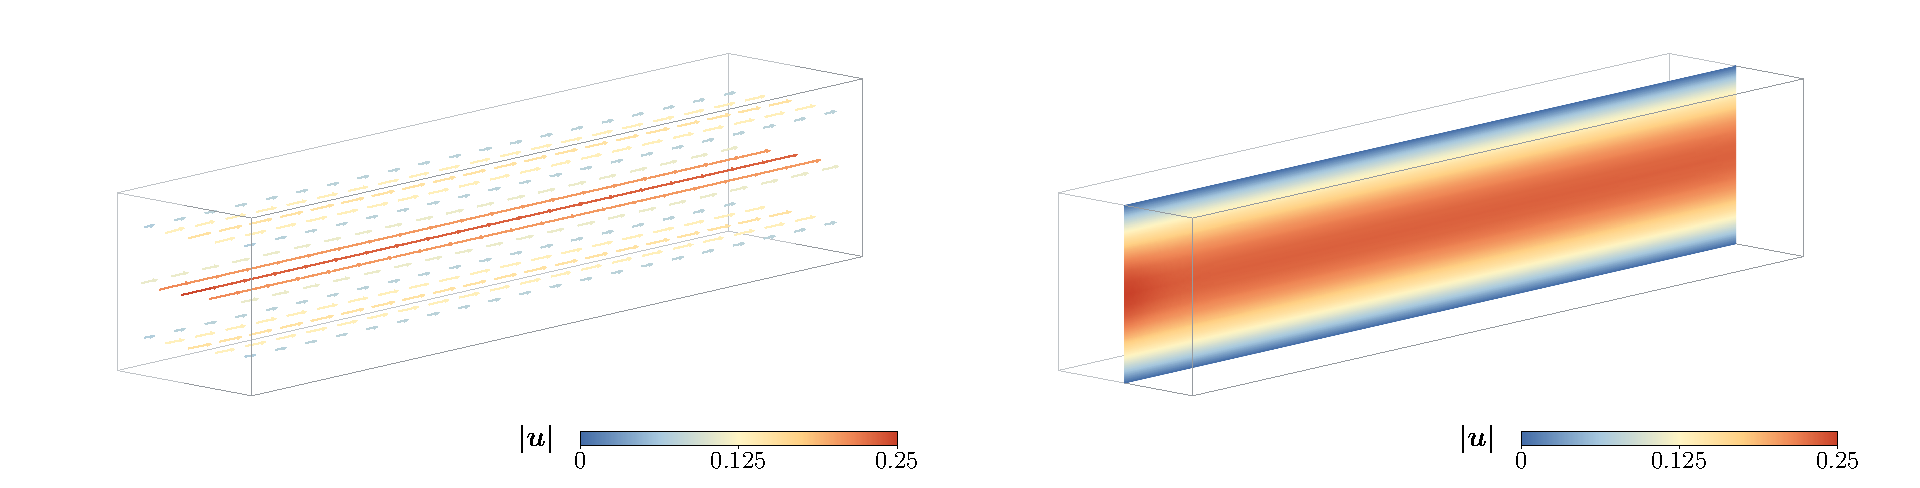
\includegraphics[width=\textwidth]{figures/applications/channel_u.pdf}
\caption{Straight-channel flow at $t=2$ on $K=12$: velocity vectors
(left) and the velocity magnitude on $z=0.1$ (right).}
\label{fig:channel-u}
\end{figure}
\begin{figure}[!htbp]
\centering
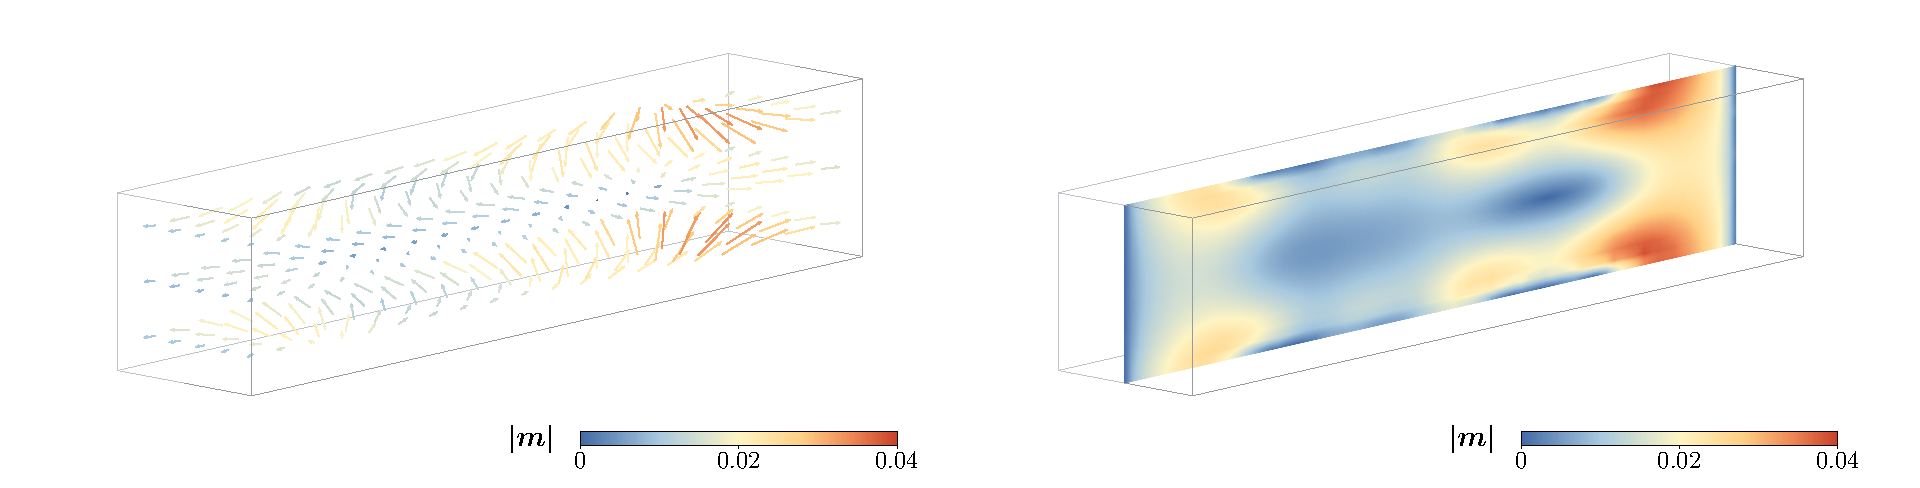
\includegraphics[width=\textwidth]{figures/applications/channel_m.pdf}
\caption{Straight-channel flow at $t=2$ on $K=12$: magnetization
vectors (left) and the magnetization magnitude on $z=0.1$ (right).}
\label{fig:channel-m}
\end{figure}
\begin{figure}[!htbp]
\centering
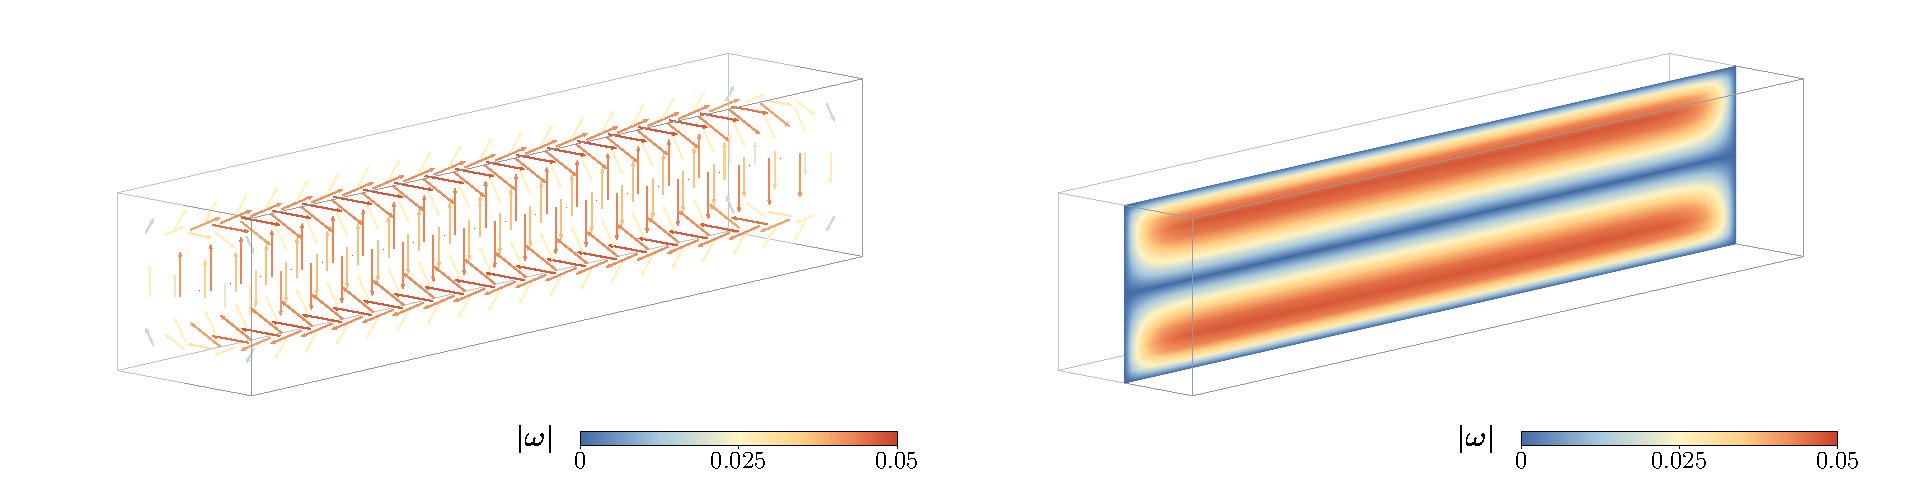
\includegraphics[width=\textwidth]{figures/applications/channel_omega.pdf}
\caption{Straight-channel flow at $t=2$ on $K=12$: particle angular
velocity vectors (left) and their magnitude on $z=0.1$ (right).
The arrows display instantaneous vectors, not particle trajectories.}
\label{fig:channel-omega}
\end{figure}
\FloatBarrier
